\section{Executable worlds for language-model agents}
\label{sec:C06:executable}
Textual agents often operate in environments whose important state can be represented symbolically: files, database records, task statuses, permissions, and tool outputs. A world model can predict this structured state instead of rendering a visual future. Executable transition rules have the advantage that invariants can be checked directly. They have the disadvantage that a missing rule or hidden service behavior can invalidate the simulation. A generated tool response should be marked as imagined so that it cannot be mistaken for an actual observation and written into persistent memory as verified fact.

The separation between hypothetical and observed events should be structural. Maintain distinct event types or stores for simulation, proposals, and executed operations. A natural-language disclaimer embedded in the same untyped text is fragile: a later summarizer may omit it. If a planner imagines that a test passes and the memory writer records only the passing result, future sessions inherit fabricated evidence. The same problem appears when synthetic training trajectories are mixed with real traces without provenance. The system must preserve whether each transition was measured, simulated by executable rules, or sampled from a generative model.

Model validation should focus on transition invariants and counterexamples. For a file-editing environment, verify that reads reflect prior writes, path resolution is consistent, and failed operations do not silently mutate state. For a workflow environment, check allowed status transitions, authorization changes, and duplicate requests. A model that predicts common successful traces may still violate these invariants on rare branches. Such failures can be more consequential than an average next-observation loss suggests because planners deliberately explore unusual sequences.

The control loop separates model-generated futures from the evidence that updates the agent. Let $H_t^o$ contain observed interaction records, $b_t=\mathcal B(H_t^o)$ be the inferred belief, and $B_t$ the planning budget. A proposal operator $\mathcal G$ returns a finite set of nonempty action sequences,
\begin{equation}
\begin{aligned}
 \mathcal P_t&=\mathcal G(b_t,B_t)
 \subseteq\bigcup_{h=1}^{H_{\max}}\mathcal A^h,\\
 \widehat\tau_t^p&\sim\widehat P_\phi(\cdot\mid b_t,p),
 \qquad p\in\mathcal P_t,\\
 \widehat J_t(p)&=\mathcal V(\widehat\tau_t^p).
\end{aligned}
\label{eq:C06:imaginedselection}
\end{equation}
The horizon limit $H_{\max}$ bounds sequence length, $\widehat P_\phi$ is the learned rollout law, and $\mathcal V$ is a declared scalar evaluation functional incorporating the available uncertainty estimate. Neither that estimate nor the score is assumed calibrated. With a declared feasibility predicate $\chi$,
\begin{equation}
\begin{aligned}
 \mathcal P_t^f&=\{p\in\mathcal P_t:\chi(p,b_t)=1\},\\
 p_t^\star&\in\argmax_{p\in\mathcal P_t^f}\widehat J_t(p),
 \qquad a_t=(p_t^\star)_1.
\end{aligned}
\label{eq:C06:feasibleplan}
\end{equation}
This selection requires $\mathcal P_t^f\ne\varnothing$ and a declared tie rule. An empty set supplies no executable action; observation, replanning, or termination requires a separately specified policy. Predicted feasibility is not current execution authority.

Let $\widetilde S_t$ be refreshed execution state, $u(a_t,\widetilde S_t)$ the current authorization predicate, and $o_\bot$ a denial observation with no submitted operation. If $K_E$ denotes the actual tool-response kernel, the observation law is
\begin{equation}
 K_u(\mathrm d o\mid a_t,\widetilde S_t)=
 \begin{cases}
 \delta_{o_\bot}(\mathrm d o),&u(a_t,\widetilde S_t)=0,\\
 K_E(\mathrm d o\mid a_t,\widetilde S_t),
 &u(a_t,\widetilde S_t)=1.
 \end{cases}
\label{eq:C06:authorizedobservation}
\end{equation}
The symbol $\delta_{o_\bot}$ denotes a point mass, not a model-predicted response. Let $\oplus$ denote record append and let $\mathcal U$ implement the inference map $\mathcal B$ incrementally on the domain of observed interaction histories, including recorded denials. Then
\begin{equation}
\begin{aligned}
 o_{t+1}&\sim K_u(\cdot\mid a_t,\widetilde S_t),\\
 H_{t+1}^o&=H_t^o\oplus(a_t,o_{t+1}),\\
 b_{t+1}&=\mathcal U(b_t,a_t,o_{t+1})
 =\mathcal B(H_{t+1}^o).
\end{aligned}
\label{eq:C06:observedupdate}
\end{equation}
The imagined trajectories $\widehat\tau_t^p$ never enter $H_{t+1}^o$ as observations. A real tool response may itself report failure or an uncertain external outcome; recording it preserves that evidence rather than certifying the described effect. The update from this actual response is the control loop's anchor. Without it, the procedure can drift into optimizing its own narratives instead of the external task.

\subsection{Current action conditioned implementations}
The inspected V-JEPA 2 repository separates passive representation training from action-conditioned robot training. Its current \path{app/vjepa_droid/train.py} exposes \path{forward_target}, \path{forward_predictions}, and \path{_step_predictor}, while the V-JEPA 2.1 training module has a distinct representation-learning path~\cite{rewrite_vjepa2_repo}. This separation matters scientifically: a stronger visual representation and a better action-conditioned transition model are related interventions, but their effects should not be conflated. The available code enables a reader to inspect where actions enter the predictor and which targets supply supervision.

The contemporary Dreamer implementation similarly exposes \path{Agent.policy}, \path{Agent.loss}, \path{imag_loss}, and \path{lambda_return} in \path{dreamerv3/agent.py}~\cite{rewrite_dreamer_repo}. These checked function names identify the distinction between real interaction, model fitting, and imagined policy learning. A current repository snapshot may differ from the cited report's experimental release; reproducing its headline results requires the original configuration as well as code. For diffusion, the inspected Diffusers \texttt{DDPMScheduler.step} and \path{add_noise} in \path{scheduling_ddpm.py} make the forward-noise and reverse-update conventions explicit~\cite{rewrite_diffusers_repo}. Swapping scheduler prediction types without changing the trained output interpretation is a concrete correctness error, not a harmless implementation variation. For example, writing $f_\theta$ for the raw model output and $\bar\alpha_t$ for the cumulative noise schedule, the scheduler's three interpretations recover different clean-sample estimates:
\begin{equation}
\begin{aligned}
 \widehat x_0^{(\epsilon)}
 &=\frac{x_t-\sqrt{1-\bar\alpha_t}\,f_\theta}
          {\sqrt{\bar\alpha_t}},\\
 \widehat x_0^{(x)}&=f_\theta,\\
 \widehat x_0^{(v)}
 &=\sqrt{\bar\alpha_t}\,x_t-\sqrt{1-\bar\alpha_t}\,f_\theta.
\end{aligned}
\end{equation}
These are alternative contracts for the trained output, not interchangeable decoders of one arbitrary checkpoint. Testing the same numeric tensor under all three modes would test a semantic mismatch rather than a solver improvement.

An integration test can hold the learned predictor fixed and replace imagined transitions with recorded real transitions for the same action sequence. The resulting oracle-transition control quantifies how much error arises in prediction versus downstream plan selection. A second ablation holds predicted transitions fixed while replacing the scorer with an independently verified objective. Neither oracle is deployable, and both must be labeled as diagnostic controls. Together they localize failures more sharply than a single final task score. They also expose a system whose representation predicts well but whose planner or reward interpretation remains wrong.

\subsection{Trace reconstruction and the scope of a simulated fact}
\label{sec:C06:traceworld}
Trace2Env's Section 4 separates an immutable reconstructed worldbook, mutable episode state, and episodic interaction memory. The worldbook retains schemas, observed transition evidence, induced rules, and provenance. An applicability gate distinguishes supporting evidence from uncertain or format-only evidence before a transition proposal reaches validation~\cite{rewrite_trace2env2026}. This addresses a concrete transfer error: an old trace can establish how a file-reading operation behaves without establishing that its particular file exists in a new episode. Reusable transition knowledge and current existence claims have different scopes.

In the pinned code, \texttt{RuntimeHarness.step} in \path{src/trace2env/runtime.py} validates candidate mutations, applies them to a copied state, checks types and verification, renders an observation, and commits through the session revision. \path{apply_mutations} and \path{check_invariants} reside in \texttt{engine.py}. An explicit \path{keep_observation} rejection policy can discard candidate effects while retaining a proposed observation~\cite{rewrite_trace2env_repo}. In this branch, due events and the step increment have already been processed; the retained candidate is the resulting working state, not necessarily the original pre-step state. The returned verification object sets its acceptance flag while carrying an \path{effects_rejected} warning. An acceptance bit alone therefore cannot be interpreted as acceptance of the proposed mutations. Preserving a fluent observation while rejecting its associated effects creates a different semantic object from a verified matching transition, and both the policy and warning must enter the experiment record.

Let $I(s)$ be a checked state invariant and $C(s,o)$ an observation-consistency predicate. A transition gate establishing $I(s')$ does not thereby establish $C(s',o')$, and neither condition proves equality with the real environment transition. A proposed successful write can leave state unchanged after effect rejection while its observation still reports completion. The pertinent test checks the returned observation against the committed state and then replays held-out actions in the real environment. Track effect rejection, observation inconsistency, and real-transition mismatch as separate outcomes. This turns a general demand for simulator fidelity into independently falsifiable interfaces.

\subsection{Generated executable worlds and learned response simulators}
\label{sec:C06:worldsynthesis}
WildAWM synthesizes replayable computer states, cross-interface tasks, and executable verifiers. Its Section 3 includes repeated state replay, agent-based checking, and quality gates for initial noncompletion, solvability, difficulty, and judgment consistency~\cite{rewrite_wildawm2026}. These are environment-construction operations: once materialized, application code and stored state execute the interaction. Qwen-AgentWorld instead trains a language model to produce environment responses through continual pretraining, supervised reasoning traces, and reinforcement learning. Its Section 3 retains masked low-information turns as context while reducing their contribution to the predictive loss~\cite{rewrite_qwenworld2026}. Both support agent learning, but their transition semantics and error sources differ.

An executable synthetic environment can be internally deterministic yet implement the wrong task semantics. A learned simulator can return a plausible response while violating a prior state commitment. Agreement among a generated verifier and model judges is valuable evidence, but shared generation assumptions can make their errors correlated. Independent checks should therefore perturb a task's initial state, remove one required effect, and alter an irrelevant field to test verifier sensitivity and specificity. For response models, replay the same action sequence after earlier writes and denials; for executable worlds, inspect reset equivalence and dependencies spanning GUI, terminal, and service interfaces.

Cost comparisons require the same boundary. Charge world construction and verifier repair to the synthesized environment, and training plus sampled response generation to the learned simulator. Then report downstream real-environment performance separately from agreement with a synthetic judge. A gain in a simulated policy's return can reflect exploitation of the simulator or verifier, so a real held-out transfer set is indispensable. The comparison should identify which component provides reliable transitions, which supplies task diversity, and which determines reward; averaging those roles into one world-model score would conceal the mechanism.



Figure~\ref{fig:C06:typed-rollout} isolates the mechanism and its stated information boundaries.
\begin{figure}[!htbp]
\centering
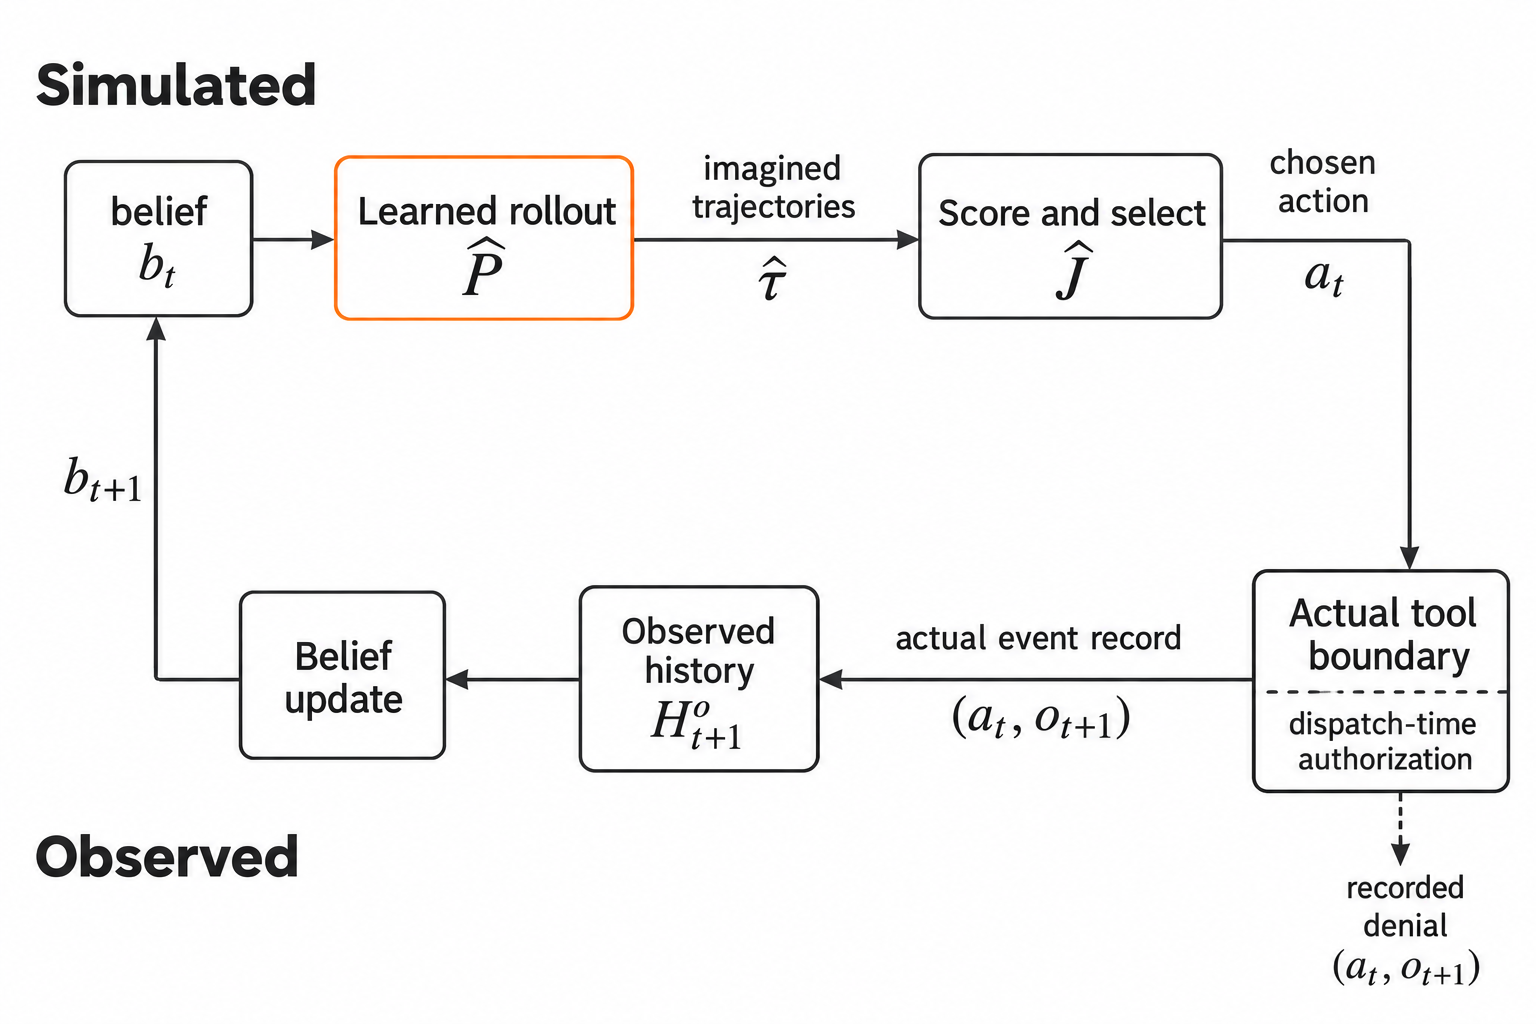
\includegraphics[width=\linewidth]{book/figures/assets/F06review.png}
\caption{Model-generated futures and observed interaction have different evidential types. Candidate rollouts and scores guide selection; the actual attempted-action/response record updates $H_{t+1}^o$ and the belief derived from it. The tool boundary checks current authority and can return denial without dispatch. An observed response can still leave an external effect uncertain. No experiment is reported. The denial note names one possible actual return, not a separate evidential history.}
\label{fig:C06:typed-rollout}
\end{figure}
